\documentclass{article}
\usepackage{tikz}
\usetikzlibrary{arrows.meta,positioning,calc,shapes.geometric}
\pagestyle{empty}
\begin{document}
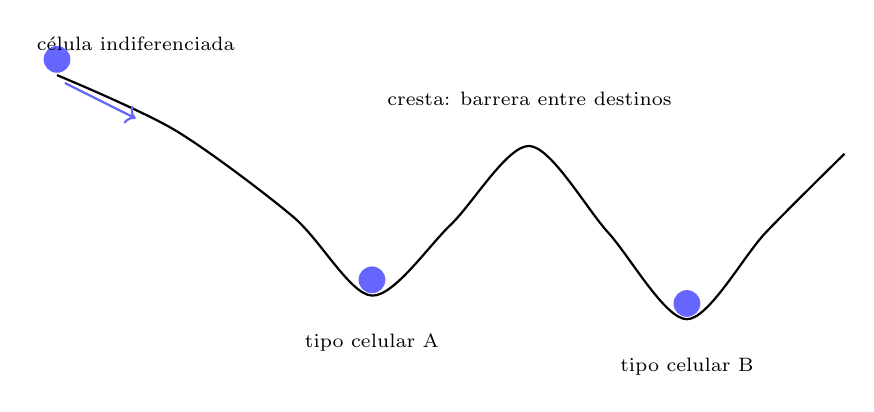
\begin{tikzpicture}

\draw[thick] plot[smooth] coordinates {(0,4.2) (1.5,3.5) (3,2.4) (4.0,1.4) (5.0,2.3) (6.0,3.3) (7.0,2.2) (8.0,1.1) (9.0,2.2) (10.0,3.2)};
\fill[blue!60] (0.0,4.4) circle (0.17); \node[font=\scriptsize] at (1.0,4.6) {célula indiferenciada};
\draw[->, thick, blue!60] (0.1,4.1) -- (1.0,3.65); 
\fill[blue!60] (4.0,1.6) circle (0.17); \node[font=\scriptsize, align=center] at (4.0,0.8) {tipo celular A};
\fill[blue!60] (8.0,1.3) circle (0.17); \node[font=\scriptsize, align=center] at (8.0,0.5) {tipo celular B};
\node[font=\scriptsize] at (6.0,3.9) {cresta: barrera entre destinos};

\end{tikzpicture}
\end{document}
